\chapter{Introducci\'on}\label{capit:cap1}
\vspace{-2.0325ex}%
\noindent
\rule{\textwidth}{0.5pt}
\vspace{-5.5ex}% 
\newcommand{\pushline}{\Indp}% Indent puede ir o no :p

La interacción entre humanos se lleva a cabo gracias a la comunicación  que existe entre ellos, esta puede ser oral o escrita y generalmente viene acompañada de gestos realizados con la cara, manos o otra cualquier parte del cuerpo. 
Estos gestos sirven como complemento de la comunicación pues ayudan a que el mensaje sea percibido de manera correcta.

El creciente desarrollo de la tecnología, a llevado  a crear y estudiar distintas áreas de las ciencias computacionales, particularmente el área de interacción humano computadora (HCI, por sus siglas en ingl\'es Human Computer Interaction), la área encargada del estudio y diseño de la forma en que el humano interactua con la computadora. 
Uno de los objetivos principales de esta área es que la interacción se lleve acabo de manera natural. 
No resulta extraño que los investigadores de HCI se hayan interesado en los gestos corporales, en especial los gestos realizados con las manos, para crear un ambiente natural entre el usuario y la computadora.  
Por lo que es necesario que la computadora pueda identificar la o las manos del usuario y reconocer el gesto que este realiza. 

A finales de los años noventa se empezar\'on a desarrollar t\'ecnicas para  el reconocimiento de gestos con las manos. Los primeros acercamientos utilizaban como medio de captura sensores como: guantes de datos, marcadores de colores y acelerómetros; los cuales se colocaban en la o las manos para poder capturar la posición e identificar la pose realizada. 
Las técnicas desarrolladas posteriormente obtienen la información necesaria para reconocer el gesto usando distintos tipos de imágenes o vídeos, que son obtenidos mediante diversos tipos de cámaras.

Los métodos que utilizan imágenes o vídeo son los más utilizados para realizar el conocimiento de los gestos ya que la interacción entre el usuario y la computadora es más natural, el inconveniente con estos métodos es que es un problema difícil de resolver pues existen distintas variables que entran en juego para obtener una buena precisión en el reconocimiento. 

Aunque existe gran variedad de métodos y sistemas que hacen el reconocimiento de gestos de las manos no existe alguno que el reconocimiento tenga un alto grado de precisión en todas las situaciones que se presentan en el mundo real.  

Es por eso que se propone crear un sistema que reconozca gestos realizados con las manos, en situaciones que presentan baja iluminación y cuando existe oclusión de los dedos. 
El sistema se enfoca en atacar estos problemas cuando las manos no se encuentran en movimiento, pero también se abordar\'an los gestos con las manos que involucran movimiento. El objetivo del sistema es mostrar que se obtiene mayor precisión en el reconocimiento de los gestos utilizando como medio de captura dos sensores Kinect.   



\section{Definici\'on del problema}\label{sec:DefinicionProblema}

Existen diversas técnicas que logran obtener buena precisión en el reconocimiento de gestos realizados con las manos, pero no hay técnicas que tengan buena precisión y que al mismo tiempo se adecuen a todo tipo de situaciones que se presentan en la vida real como: amigable con el usuario, invariante a la iluminación, rotación, al fondo, que funcione en tiempo real o cuando exista oclusión.



\section{Justificaci\'on}\label{sec:Just}

Debido a la complejidad del problema de reconocimiento de gestos con las manos, las técnicas desarrolladas y actuales se enfocan en aspectos específicos para obtener un buen grado de precisión. De manera que se necesitan nuevos métodos que aborden los aspectos dejados de lado y funcionen no solo en condiciones ideales si no en situaciones que se presentan de manera natural y al mismo tiempo se obtenga un alto grado de precisión.  

Una vez logrado lo anterior se pueden desarrollar nuevas aplicaciones y tecnologías que ayuden a interactuar con naturalidad al usuario y la computadora.



\section{Objetivo general}\label{sec:ObjetivoGeneral}
 
Desarrollar un sistema que permita controlar la computadora haciendo uso de gestos con las manos, estáticos y dinámicos. El sistema debe ser robusto, funcionar en circunstancias de baja iluminación, cuando exista oclusión en gestos dinámicos.



\section{Objetivos espec\'ificos}\label{sec:objetivosEspecificos}

\begin{itemize}
	\item Identificar los m\'etodos actuales de reconocimiento de gestos, estáticos y din\'amicos cuando existe baja iluminación  y cuando existe oclusión. 
	
	\item  Obtener conocimiento acerca del funcionamiento de sistema Microsoft Kinect.
	
	\item Desarrollar un sistema de reconocimiento de gestos estáticos y dinámicos, fusionando la información de los sensores de  profundidad de dos dispositivos kinect. El sistema desarrollado deberá funcionar en circunstancias de baja iluminación y también cuando existe oclusión, causada por los dedos. 
	
	\item Analizar el sistema dise\~nado, en cuanto a su eficiencia presentada en base al reconocimiento de los gestos, en circunstancias de baja iluminación y oclusión. En el análisis del sistema se usar\'a información real.  
	
	\item Comparar y analizar el modelo propuesto haciendo uso de uno y dos dispositivos Kinect. 
\end{itemize}


\section{Limitaciones y suposiciones}\label{sec:Limitaciones&Suposiciones}

Gran porcentaje de los trabajos previos en el \'area de reconocimiento de gestos con las manos basados en el modelo de la visión  utilizan c\'amaras digitales o c\'amaras web. Esta investigación utiliza dos dispositivos Kinect, para obtener la información de entrada del sistema.

De  manera que las limitaciones del sistema propuesto están dadas por las características de dicho dispositivo, tales como la distancia  a la que se encuentran los dispositivos con el usuario y la resolución del sensor. 

Otra limitante es el número de gestos que podrá reconocer el sistema.



\section{Reconocimiento de gestos con la manos}\label{sec:ReconocimientoGestos} 

La definición de gestos \citep{Mitra2007} son movimientos del cuerpo expresivos y significativos que involucran a los dedos, manos, brazos, cabeza, cara o cuerpo con la intención de transmitir información relevante o de interactuar con el ambiente.

Los primeros acercamientos para llevar acabo el reconocimiento de gestos con las manos fue usando modelos de contacto \citep{Rautaray2012} y \citep{Nayakwadi2014}, como su nombre lo dice utilizan dispositivos que est\'an en contacto f\'isico con la mano del usuario \ref{fig:Modelos:1}, para capturar el gesto a reconocer, por ejemplo existen guantes de datos, marcadores de colores, acelerómetros y pantallas multi-touch, aunque estos no son tan aceptados pues entorpecen la naturalidad entre la interacción del humano y la computadora. Los modelos basados en la visión \ref{fig:Modelos:2} , surgieron como respuesta a esta desventaja, estos utilizan cámaras para extraer la información necesaria para realizar el reconocimiento, los dispositivos van desde cámaras web hasta algunas más sofisticadas por ejemplo c\'amaras de profundidad.   

\begin{figure}[h!]
\begin{center}
\subfigure [Dispositivos basados en contacto: en la parte izquierda de la imagen se observan los guantes de datos \protect\footnotemark{}
, en el centro los guantes de colores  \protect\footnotemark{}  y a la derecha se encuentra el dispositivo wii \protect\footnotemark{} . \addtocounter{footnote}{-3}]
{
    {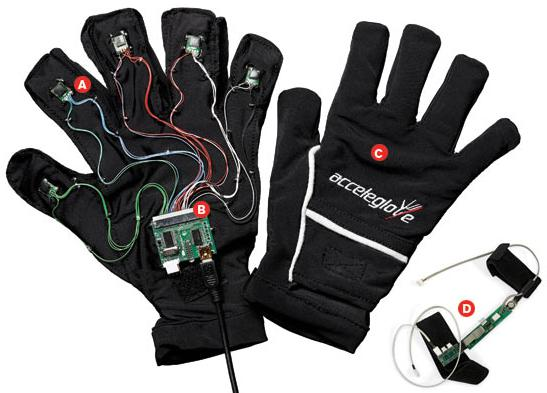
\includegraphics[scale=.25]{./Figures/Dataglove.jpg}}  \qquad
	{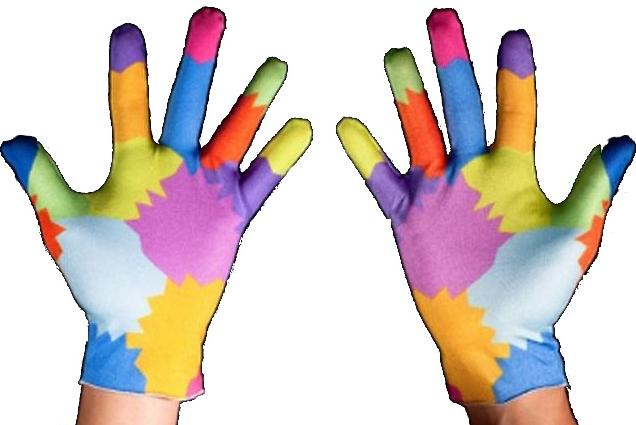
\includegraphics[scale=.25]{./Figures/colorGloves.jpg}} \qquad   	
	{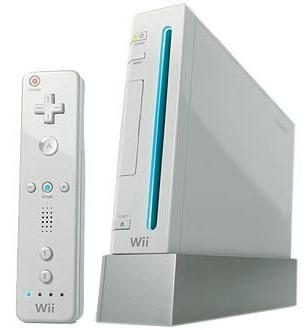
\includegraphics[scale=.29]{./Figures/wii.jpg}} 	  	
	\label{fig:Modelos:1}
}
\subfigure [Dispositivos basados en visión: en la imagen se observan distintos tipos de cámaras en la parte izquierda de la imagen se observa una web \protect\footnotemark{}, en el centro una digital \protect\footnotemark{} y a la derecha de la imagen una TOF \protect\footnotemark{} .]
{
	{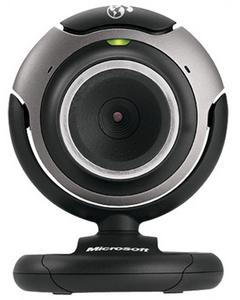
\includegraphics[scale=.3]{./Figures/webcam.jpg}} 		\qquad
	{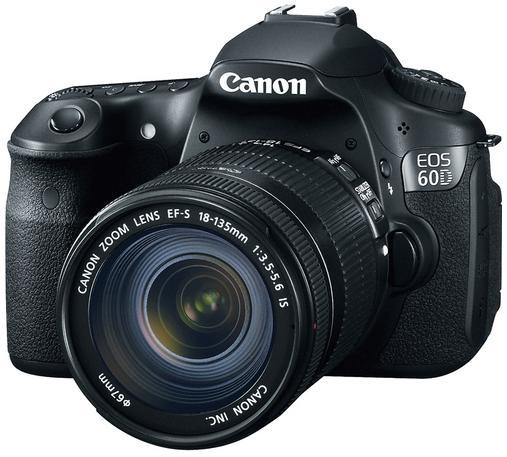
\includegraphics[scale=.2]{./Figures/digitalCamera.jpg}}  \qquad
	{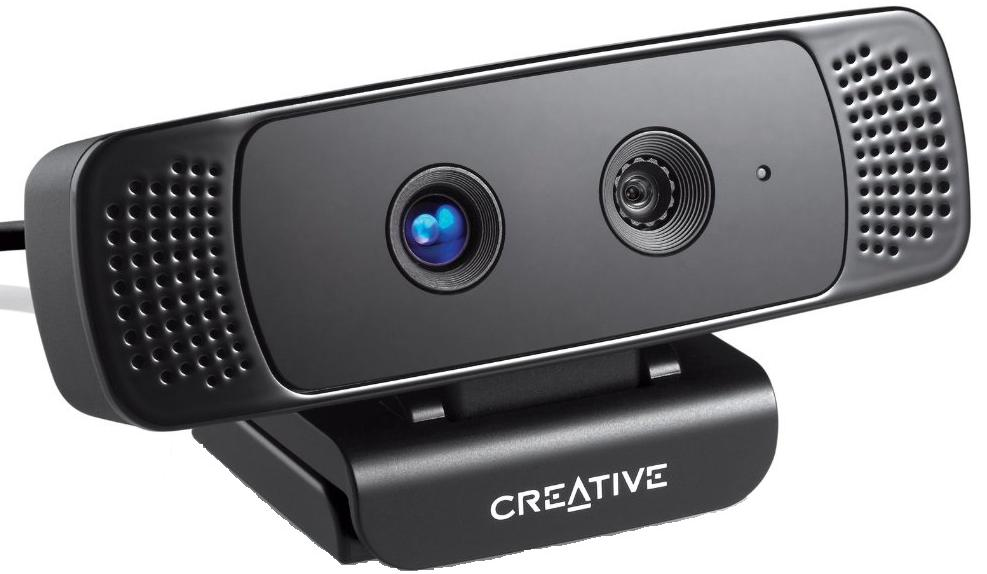
\includegraphics[scale=.15]{./Figures/TOF.jpg}} 
    \label{fig:Modelos:2} 
}
\caption{Dispositivos utilizados para la captura de gestos.} 
\label{fig:Modelos} 
\end{center}
\end{figure} 


\footnotetext[1] {\url{ http://www.technologyreview.com/article/414021/open-source-data-glove/}} \stepcounter{footnote}
\footnotetext[2] {\url{http://www.digitaltrends.com/computing/the-gloves-that-could-change-the-world/}}
\footnotetext[3] {\url{https://www.nintendo.es/Wii/Wii-94559.html}}

\footnotetext[4] {\url{http://es.ccm.net/download/descargar-2562-driver-de-microsoft-lifecam-vx-3000}}
\footnotetext[5] {\url{http://www.canon.com.mx/ficha.aspx?id=722}} 
\footnotetext[6] {\url{http://us.creative.com/p/web-cameras/creative-senz3d}}

En este trabajo, se toma el enfoque basado en la visión ya que se quiere obtener un sistema que para el usuario la interacción sea natural y la manera de lograrlo es tomando este enfoque.  



\section{Estado del arte}\label{sec:EstadoDelArte} 

La sección anterior explica los modelos utilizados para llevar acabo el reconocimiento de gestos con las manos, enseguida se presentan los trabajos relevantes de cada uno de estos enfoques y también se mencionan algunos de los sistemas comerciales importantes. 

\subsection{Modelos de contacto}
 
Como se menciono en la sección anterior los primeros trabajos de reconocimiento de gestos con las manos utilizaba este modelo, actualmente se sigue utilizando pero en menor grado. En los párrafos siguientes se presentan dos trabajos relevantes en esta área. 

El primer trabajo que se presenta es el realizado por \citep{Yoon2012} el cual propone un sistema de reconocimiento de gestos estáticos usando un guante de datos, el cual reconoce $24$ gestos tomados del Lenguaje de Señas Americano, ASL (por sus siglas en inglés, American Sign Lenguaje). Este modelo consta de tres etapas, las cuales se explican enseguida. 

La primera etapa del sistema consiste en capturar la información proporcionada por un guante de datos, la cual esta siendo enviada por un protocolo de control de transmisión TCP, (por sus siglas en inglés, Transmission Control Protocol). 
 
Una vez que la información es recibida, los datos son pre-procesados, es decir son normalizados y las características son extraídas, las características son las correlaciones que existe entre los ejes.    
 
La clasificación de gesto se realiza con un modelo de mezclas adaptativo. Para entrenar el modelo de mezclas se toman datos de $5$ personas, $300$ muestras de cada gestos, $8000$ por cada participante. Se realizaron pruebas con estos mismos datos; con un sujeto se alcanzó una precisión de $93.38 \%$ con los demás participantes se obtuvo una precisión de $89.97 \%$.  

La principal desventaja del sistema es que baja la precisión cuando se cambia de usuario, aunque después se adapta y mejora la precisión, otra desventaja para este sistema es que solo reconoce gestos estáticos. 

A finales del año 2014 se lanzó el dispositivo MYO \footnote{\url{https://www.thalmic.com/en/myo/}}, el cual reconoce gestos dinámicos, los detalles del dispositivo se encuentran en ultima parte de esta sección. 


\subsection{Modelos basados en la visión}   

Este modelo es el más popular debido a la variedad de sus aplicaciones y la diversidad de cámaras existentes que proporcionan distinto tipo de información la cual puede hacer que el reconocimiento tenga mayor precisión. Enseguida se presenta tres  trabajos relevantes los cuales utilizaron distintos tipos de cámaras y número de ellas. 

%En el trabajo propuesto por \cite{Premaratne2013} realizan un modelo de reconocimiento de gestos estático y dinámico basados en el algoritmo de Lucas-Kanade. Las principales ventajas de este método son que es invariante a rotación, escala y al fondo. Aunque el modelo es afectado por los cambios en la iluminación.
%::::::::::::::::::::::::::::::::::::::::::::::::::::::::::::::::::::::::::::::::::::::::::::::::::::::::

En trabajo de \citep{Huang2011}, propone un método que reconoce $11$ gestos estáticos y dinámicos, la aportación del trabajo es la segmentación de la mano que se lleva acabo usando filtros de Gabor. El sistema propuesto utiliza una cámara CCD para obtener la información de entrada. El sistema es robusto a la iluminación. 
 
Antes de hacer la segmentación de la mano se le aplica a la imagen un preprocesamiento que consiste en aplicar un filtro de Gabor, después se escoge uno de los tres modelos del color; YCbCr, Gaussiano o Soriano, tomando en cuenta un nivel de gris.  
Una vez que es realizado el preprocesamiento el paso siguiente es segmentar la mano del antebrazo para esto se hace un barrido de la imagen por filas. Se segmenta la mano tomando en cuenta la distancia que existe entre la parte superior de la imagen y el número máximo de pixeles de un solo valor (el valor mayor del histograma).

Una vez realizada la segmentación el siguiente paso es obtener las características necesarias para el reconocimiento, las características son obtenidas utilizando análisis de componentes principales, PCA (por sus siglas en inglés, Principal Component Analysis).\\
La clasificación la hacen usando maquinas de vectores de soporte, SVM (por sus siglas en inglés, Support Vector Machines).   

La precisión del reconocimiento varía dependiendo de las imágenes, si son reales o si se les aplica antes un filtro de Gabor, también cambia si el usuario usa manga corta o larga.  
Las principales ventajas son que el sistema funciona con cambios en la iluminación y es robusto a la rotación y escala. La desventaja es que el problema de oclusi\'on no es tratado. 

%:::::::::::::::::::::::::::::::::::::::::::::::::::::::::::::::::::::::::::::::::::::::::::

Por otra parte en el trabajo propuesto por \citep{Caputo2012} gestos dinámicos y estáticos son reconocidos, estos últimos son utilizados para determinar el inicio y el término de los gestos dinámicos. Se utilizan dos sensores Kinect y una cámara web Logitech C910 de alta definición para capturar los gestos. El trabajo esta compuesto de cuatro etapas, las cuales se explican enseguida. 

La primera es la configuración de los dispositivos de captura de datos del sistema. Los dos sensores Kinect son calibrados entre ellos para generar un sistema de coordenadas que esta basado en la ubicación de la  manos y la cabeza. La cámara y los dispositivos Kinect no son sincronizados entre si.  

La parte de la detección y seguimiento, se lleva acabo utilizando la librería OPENNI, en específico usando la detección del esqueleto proporcionado por esta librería. El esqueleto nos proporciona el punto de la palma de la mano por la cual la región de interés, ROI (por sus siglas en inglés, Region of Interest) es seleccionada, para tener la localización exacta de la mano, se utiliza la cámara RGB. La localización de la mano se realiza convirtiendo la imagen en una imagen binaria, usando un umbral que es determinado por el espacio del color HSV (Matiz, Saturación, Valor); son utilizados guantes neón color rosa o verde para ubicar con mayor facilidad las manos.   

Una vez obtenida la imagen binaria se calcula el contorno de la mano usando el algoritmo de Chang y Chen, dicho contorno es extraído como polígono y  es simplificado con el algoritmo de Douglas Peuker. 

El reconocimiento del gesto se basa en empatamiento de polígonos, basados en la distancia de dos polígonos. Esto usando Distancia de momentos HU (Hu-moments distance) y ángulo de giro (turning angle). 
Los gestos 3D son calculados usando la diferencia de las posiciones de la mano, en cada cuadro. Las fórmulas para calcular estos gestos depende de que gesto se  realice.  
Para probar la precisión del sistema se crearon dos bases de datos, una con $120$ polígonos etiquetados que representan $11$ gestos y otra con $144$ gestos de $3$ personas distintas realizando los $11$ gestos. La precisión obtenida usando la distancia de ángulo de giro es de $85 \%$, usando la distancia de momentos HU la precisión es de $58 \%$.  

%::::::::::::::::::::::::::::::::::::::::::::::::::::::::::::::::::::::::::::::::::::::::::::::::::::::::

Otra aportación importante fue hecha por \citep{Kang2013} ellos proponen un sistema de reconocimiento de  gestos estáticos utilizando el sensor Kinect como dispositivo de captura de los gestos. El sistema reconoce $24$ gestos, los cuales pertenecen al ASL, el reconocimiento es realizado en cuatro etapas, las cuales se explican a continuación.  

En la primera etapa la imagen es capturada y la mano junto con el antebrazo son segmentados del fondo. Las imágenes de entrada del sistema son proporcionadas por el sensor de profundidad del Kinect, la mano es detectada usando el SDK (Software Developmet Kit) del Kinect, que proporciona el punto de la palma de la mano, la región de interés es seleccionada usando este punto, donde  solo se encuentra la mano y parte del antebrazo.   

El siguiente paso es extraer las características, las cuales son extraídas usando Histogramas Orientados a Gradientes, HOG (Histogram of Oriented Gredient).  

El paso siguiente es clasificar los gestos, se utiliza el algoritmo de aprendizaje de máquina, máquinas de soporte vectorial.\\
Para el entrenamiento del se utilizaron $2400$ imágenes, $100$ por cada letra del alfabeto. Se encontró que existe gesto ambiguos, es decir que no se pueden clasificar correctamente, estos son los gestos que representan la letras A, E, M, N, S, T. 
Se realizo una prueba en linea, donde los gestos aparecían aleatoriamente para ser clasificados. La precisión de todos los gestos se encuentra alrededor de $92.8 \%$, pero el de los gestos ambiguos es $72.9 \%$

Por ultimo una interfaz gráfica es mostrada donde se aprecia el reconocimiento de los gestos en tiempo real.  

%::::::::::::::::::::::::::::::::::::::::::::::::::::::::::::::::::::::::::::::::::::::::::::::

%La SECCIÓN A pesar que la mayoría de los modelos vistos en la parte de arriba solucionan muchos de los problemas de los modelos basados en la visi\'on. Ninguno de ellos puede resolver el problema de iluminaci\'on y oclusi\'on, formada por lo dedos. All\'i la importancia de la investigaci\'on propuesta, pues dar\'a soluci\'on a estos inconvenientes al momento de reconocer los gestos.
 
\subsection{Sistemas comerciales}

Existen dispositivos como: Leap Motion \footnote{\label{LeapMotionFN} \url{https://www.leapmotion.com/}}, MYO \footnote{\label{MyoFN}  \url{https://www.myo.com/}}, y software como: Flutter \footnote{\label{FlutterFN} \url{ https://flutterapp.com/}}, que realizan el reconocimiento de gestos, y este reconocimiento es aplicado para controlar la computadora. Algunos de estos dispositivos comerciales tienen  buen rendimiento en cuanto a la precisión y a sobrellevar los problemas del reconocimiento de gestos, el inconveniente es que los desarrolladores de los dispositivos o software no dan a conocer los detalles de como solucionan algunos de los problemas o como mejoran la precisión. \\ 
Enseguida se describen los sistemas mencionados anteriormente.
 
El dispositivo Leap Motion, fig \ref{fig:LeapMotion} fue creado para el seguimiento de manos y dedos, este también hace el reconocimiento de ciertos gestos estáticos y dinámicos. El dispositivo consta de tres emisores y dos cámaras infrarrojas, estos sensores capturan los datos crudos en un rango de $60 \times 60 \times 60$ $cm.$ y con la información capturada se construye un modelo 3D de las manos \citep{Weichert2013}. 

\begin{figure}[h!]
\begin{center}
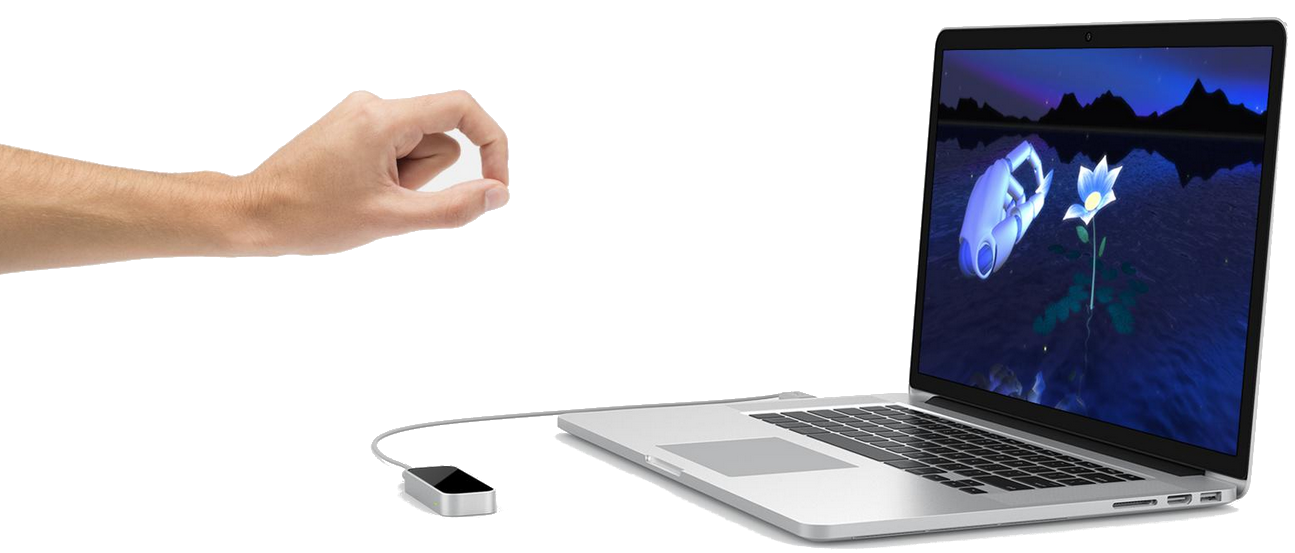
\includegraphics[scale=.3]{./Figures/LeapMotion.png}
\end{center}
\caption{Ejemplo del reconocimiento del gesto usando Leap Motion, mostrando mediante una aplicación donde los gestos son representados en 3D, que es el dispositivo que se encuentra conectado a la Laptop. Imagen recuperada de \ref{LeapMotionFN}.}
\label{fig:LeapMotion}
\end{figure}

El proceso de como se capturan los datos, la segmentación, la extracción de características, el seguimiento y el reconocimiento del dispositivo no se conoce a detalle.\\ 
Solo se conoce \footnote{ \url{http://blog.leapmotion.com/hardware-to-software-how-does-the-leap-motion-controller-work/}} que se utilizan tres cámaras infrarrojas, con la imágenes obtenidas con se hace una representación 3D de las manos, antes de realizar el modelo las imágenes son segmentadas del fondo para eliminar el ruido generado por la iluminación u otros objetos que causen ruido en la imágenes. \\
Para realizar el seguimiento se extraen la características, una de ellas son el dedos, el algoritmo de seguimiento interpreta la información 3D e infiere la posición de los objetos ocluidos. Se aplican filtros para suavizar los datos. 


Un dispositivo de reconocimiento de gestos basado en el modelo de contacto, es el MYO, este aparato es un brazalete que reconoce $5$ gestos dinámicos. Leyendo la actividad de los músculos del antebrazo y mandando estas señales vía Bluetooth a la computadora donde estas señales son procesadas. \footnote{\url{http://www.digitaltrends.com/pc-accessory-reviews/myo-gesture-control-armband-review/}} 

No se cuenta con la informacion detallada del funcionamiento de MYO, lo único que se conoce es que el reconocimiento consta de tres etapas \footnote{\url{https://www.quora.com/How-does-MYO-wearable-gesture-control-work}}. La primera es la adquisición de la señales eléctricas que producen los músculos del antebrazo, las cuales son capturadas mediante sensores EMG (estos detectan la actividad eléctrica), giroscopio, acelerómetro y magnetómetro; en la segunda etapa se amplifica la señal y se aplica un filtro pasa banda. Por último se realiza el procesamiento de la señal donde se reconoce el gesto usando un algoritmo de aprendizaje de máquina desarrollado por la compañía.  

\begin{figure}[h!]
\begin{center}
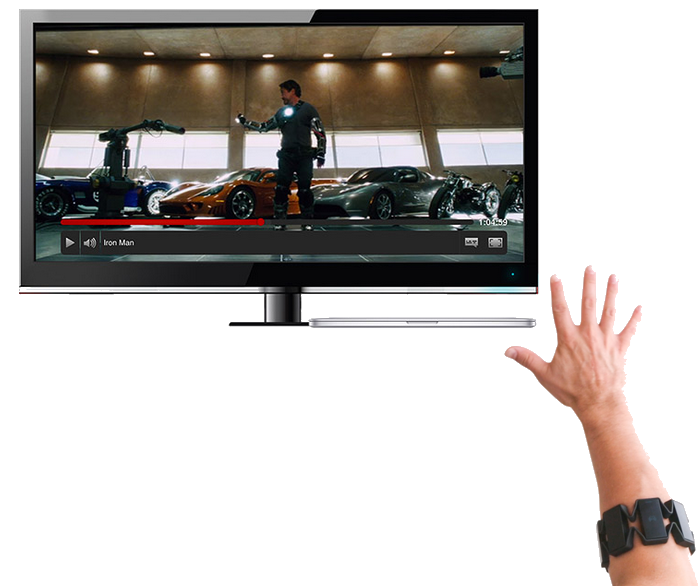
\includegraphics[scale=.5]{./Figures/MYO.png}
\end{center}
\caption{Ejemplo del reconocimiento del gesto usando MYO, controlando el volumen de la computadora. El dispositivo es el aparece en el brazo del sujeto. Imagen recuperada de \ref{MyoFN}.}
\label{fig:Myo}
\end{figure}

MYO funciona en cualquier ambiente donde haya variaciones en la iluminación y es invariante a rotación. La desventaja que tiene la calibración pues esta puede ser tediosa ya que requiere realizar repeticiones de algunos gestos y esta requiere de varios intentos; el use del dispositivo requiere uso de manga corta; otra desventaja es que tiene una cantidad considerable de falsos positivos. \footnote{ \url{http://myogroupfive.blogspot.mx/2013/11/benefits-disadvantages-for-business\_ 24.html}} 


Enseguida se explica el software de reconocimiento de gestos estáticos Flutter, fig:\ref{fig:Flutter} el cual reconoce cuatro gestos estáticos usando la cámara web como dispositivo de entrada. 

Se conoce muy superficialmente como funciona el software, pues solo se sabe que la mano es detectada por la cámara, para que la detección sea correcta la mano tiene que estar totalmente frente a la cámara web. Los algoritmos utilizados para el reconocimiento no se conocen.  
\begin{figure}[h!]
\begin{center}
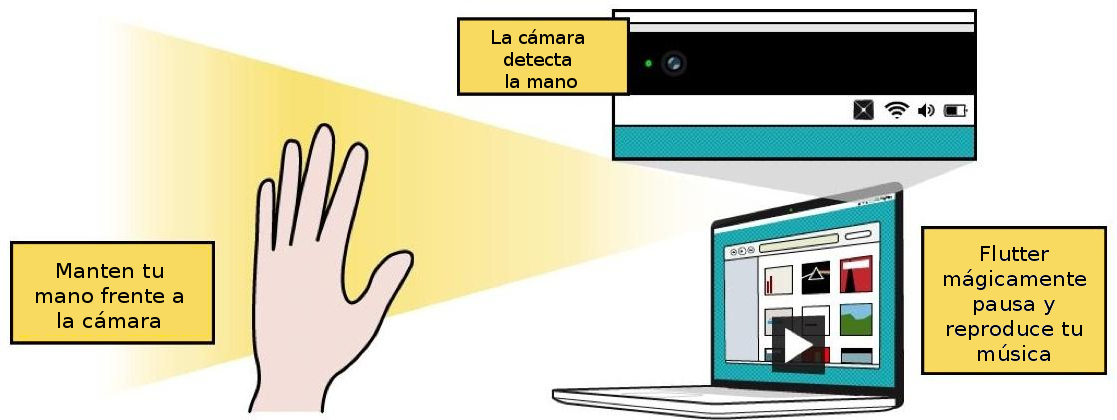
\includegraphics[scale=.4]{./Figures/Flutter.jpg}
\end{center}
\caption{La imagen anterior representa el funcionamiento del software Flutter. Imagen recuperada de \ref{FlutterFN} .}
\label{fig:Flutter}
\end{figure}

Flutter permite controlar aplicaciones multimedia como: YouTube \footnote{\url{https://www.youtube.com/}} ,VLC \footnote{\url{http://www.videolan.org/vlc/}}, Spotify \footnote{\url{https://www.spotify.com/}}, Netflix \footnote{\url{https://www.netflix.com/}}. Las limitaciones del software son que solo reconoce gestos estáticos, realiza acciones no deseadas al hacer gestos involuntarios y no siempre reconoce los gestos.  

%::::::::::::::::::::::::::::::::::::::::::::::::::::::::::::::::::::::::::::::::::::::::::::::::::::::::: 

Aunque estos dispositivos y software para reconocer gestos solucionan algunos problemas importantes en el área, sigue existiendo el problema de oclusiones e iluminación.
De allí la importancia que existan nuevos modelos que ataquen estos problemas que se presentan frecuentemente en el reconocimiento de los gestos.
  
\section{Organizaci\'on de la tesis}\label{OrganizacionTesis}

La tesis se encuentra distribuida de la siguiente manera: la segunda sección presenta los fundamentos teóricos como base para la comprensión del tema. La tercera sección presenta la metodología utiliza en el sistema propuesto. En la cuarta sección se encuentran los detalles de la implementación del sistema. En la quinta sección están las pruebas realizadas al sistema junto con los resultados y las discusiones de estos. Finalmente la sexta sección presenta las conclusiones generales del sistema y el trabajo futuro. 

